\chapter{Dinamica}

Passiamo ora a studiare la dinamica, ovvero le relazioni fra forze e movimenti.

Il modello dinamico del manipolatore può essere determinato seguendo due diversi approcci: equazioni di Lagrange oppure equazioni di Newton-Eulero. Dal punto di vista della derivazione le prime sono più semplici, mentre per quanto riguarda la computazione le seconde permettono algoritmi ricorsivi efficienti. Noi vedremo solo la definizione Lagrangiana.



\section{Lagrangiana ed equazioni di Eulero-Lagrange}

La \textbf{Lagrangiana} $\mathcal{L}$ di un sistema è data dalla differenza tra la sua energia cinetica totale $\mathcal{T}$ e la sua energia potenziale totale $\mathcal{U}$:
$$
\mathcal{\bm{L = T - U}}
$$
essa è funzione delle coordinate generalizzate usate per descrivere la posizione del sistema, nonché delle loro derivate rispetto al tempo. Nel caso di un manipolatore le variabili giunto qi possono essere assunte come coordinate generalizzate. 

Le equazioni di Eulero-Lagrange, che descrivono il comportamento dinamico del sistema, sono date da:
$$
\frac{d}{dt}\left(\frac{\partial \mathcal{\bm{L}}}{\partial \dot{\bm{q}}_i}\right)
-
\frac{\partial \mathcal{\bm{L}}}{\partial \bm{q}_i}
=
\mathcal{\bm{F}}_i
\qquad
i = 1, \dots, n
$$
dove $\mathcal{\bm{F}}_i$ è la i-esima forza generalizzata, non conservativa (associata a $\bm{q}_i$).



\subsection{Energia cinetica}

L’energia cinetica totale di un manipolatore con $n$ giunti (e $n + 1$ bracci rigidi, ma il braccio di base $b_0$ non dà contributo, essendo fisso) è data dalla somma delle energie cinetiche $\mathcal{T}_{l_i}$ di ciascun braccio a cui vanno sommati i contributi $\mathcal{T}_{m_i}$ associati agli $n$ attuatori (motori) che muovono i giunti:
\begin{equation}\label{eq:kin_energy_sum}
\mathcal{T} = \sum_{i=1}^n \mathcal{T}_{l_i} + \mathcal{T}_{m_i}
\end{equation}


\subsubsection{Energia cinetica dei bracci}
Partiamo dalla seguente formulazione:
$$
\mathcal{T}_{l_i}
=
\frac{1}{2} m_{l_i} \bm{\dot{p}}_i^T \bm{\dot{p}}_i
+
\frac{1}{2} \bm{\omega}_i^T {}^b\bm{R}_i {}^i\bm{I}_{l_i} ({}^b\bm{R}_i)^T \bm{\omega}_i
$$
dove le velocità (traslazionali e rotazionali) sono indicate rispetto al centro di massa del braccio, e $\bm{I}_{l_i}$ rappresenta il tensore di inerzia del braccio $i$.


\begin{proof2}
Dalla definizione fisica:
$$
\mathcal{T}_{l_i}
=
\frac{1}{2} \int_{V_{l_i}} \underbrace{\bm{\dot{p}}_i^T \bm{\dot{p}}_i}_{\textit{velocity}^2} \underbrace{\rho dV}_{mass}
$$
usando la formula della derivata di un vettore
$$
\dot{p}_i = \dot{p}_{\ell_i} + \omega_i \times r_i = \dot{p}_{\ell_i} + S(\omega)r_i
$$
sostituendo alla precedente otteniamo (skippando i calcoli, vedi slide):
$$
\mathcal{T}_{l_i}
=
\frac{1}{2} m_{l_i} \bm{\dot{p}}_i^T \bm{\dot{p}}_i
+
\frac{1}{2} \bm{\omega}_i^T \bm{I}_{l_i} \bm{\omega}_i
$$

Ora dobbiamo però notare che il tensore di inerzia di un corpo rigido, rispetto al suo centro di massa, è costante solo se espresso in un sistema di riferimento locale solidale con il corpo ed avente origine con il centro di massa stesso.

Nel caso sopra mostrato abbiamo espresso $\bm{I}_{l_i}$ nel base-frame, e quindi non costante. Possiamo però utilizzare il tensore relativo al link-frame, trasformandolo le approriate matrici: 
$$
I_{l_i} = {}^bR_i {}^iI_{l_i} ({}^bR_i)^T
$$
dove ${}^bR_i$ è la matrice di rotazione del link-frame w.r.t base-frame.\\ Effettuando questa sostituzione abbiamo la tesi.
\end{proof2}



Ora, richiamando (\ref{eq:geom_jacob_2}), possiamo seguire lo stesso concetto e scrivere:
\begin{gather*}
\dot{\bm{p}}_{l_i}
=
\bm{J}^{(l_i)}_{p,1}\dot{\bm{q}}_1
+
\bm{J}^{(l_i)}_{p,2}\dot{\bm{q}}_2
+ \cdots +
\bm{J}^{(l_i)}_{p,i}\dot{\bm{q}}_i
=
\bm{J}^{(l_i)}_{p}\dot{\bm{q}}_i
\\
\bm{\omega}_{l_i}
=
\bm{J}^{(l_i)}_{o,1}\dot{\bm{q}}_1
+
\bm{J}^{(l_i)}_{o,2}\dot{\bm{q}}_2
+ \cdots +
\bm{J}^{(l_i)}_{o,i}\dot{\bm{q}}_i
=
\bm{J}^{(l_i)}_{o}\dot{\bm{q}}_i
\end{gather*}
dove $\bm{J}^{(l_i)}_{u,j}$ è la $j$-esima colonna di $\bm{J}^{(l_i)}_{u}$.

Queste due nuove matrici $\bm{J}^{(l_i)}_{o}, \bm{J}^{(l_i)}_{o}$ seguono un concetto analogo a quello delle colonne dello Jacobiano geometrico, però invece di far riferimento all'intero manipolatore, riguardano solo il link $i$:
\begin{itemize}
	\item Se il giunto è prismatico:
	\begin{align*}
		\bm{J}^{(l_i)}_{p,j} &= \bm{k}_{j-1} \\
		\bm{J}^{(l_i)}_{o,j} &= \bm{0}
	\end{align*}
	\item Se il giunto è rotoidale:
	\begin{align*}
		\bm{J}^{(l_i)}_{p,j} &= \bm{k}_{j-1} \times (\bm{p}_{l_j} - \bm{p}_{j-1} ) \\
		\bm{J}^{(l_i)}_{o,j} &= \bm{k}_{j-1}
	\end{align*}
\end{itemize}
per entrambi le formule valgono $\forall j = 1,\dots,i$.

Quindi, usando quest'ultime formulazioni possiamo riscrivere la forma iniziale come:
$$
\mathcal{T}_{l_i}
=
\frac{1}{2} m_{l_i} \left(\bm{\dot{q}}^T \bm{J}_p^{(l_i)T}\right) \left(\bm{J}_p^{(l_i)} \bm{\dot{q}}\right)
+
\frac{1}{2} 
\left(\bm{\dot{q}}^T \bm{J}_o^{(l_i)T}\right)
\left( {}^b\bm{R}_i {}^i\bm{I}_{l_i} ({}^b\bm{R}_i)^T \right)
\left(\bm{J}_o^{(l_i)} \bm{\dot{q}}\right)
$$

Alla fin fine, però questa formulona non è altro che 
$$
\frac{1}{2} \bm{\dot{q}}^T \textit{roba}(\bm{q}) \bm{\dot{q}}
=
\frac{1}{2}m\bm{v}^2
$$
ovvero l'energia cinetica.




\subsubsection{Energia cinetica dei motori}

Un ragionamento analogo può essere fatto per i motori. Inanzitutto supponiamo che il motore $i$-esimo che attua il giunto $i$ sia localizzato sul braccio $i-1$, come mostrato in fig. \ref{fig:dynamics1}.
\begin{figure}[H]
	\centering
	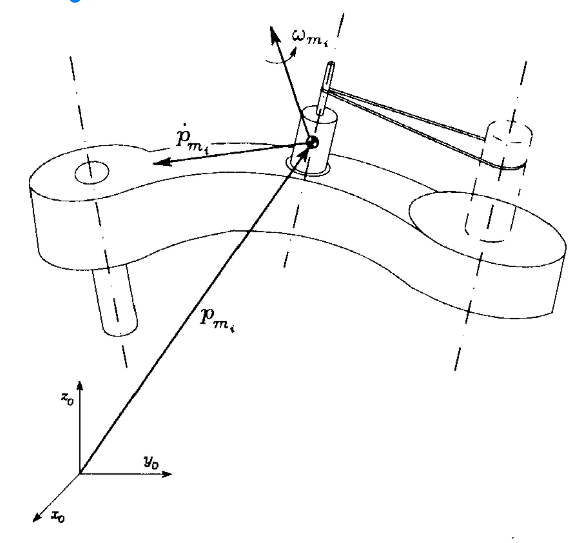
\includegraphics[width=0.3\linewidth]{images/dynamics_1}
	\caption{Posizionamento motore}
	\label{fig:dynamics1}
\end{figure}
Inoltre, per semplicità supponiamo che il contributo delle trasmissioni (gears) possa essere incluso nel motore stesso e che non ci siano movimenti indotti (i.e. il giunto i non muove altri giunti).

Quindi, analogamente ai bracci:
$$
\mathcal{T}_{m_i}
=
\frac{1}{2} m_{m_i} \bm{\dot{p}}_i^T \bm{\dot{p}}_i
+
\frac{1}{2} \bm{\omega}_i^T {}^b\bm{R}_i {}^i\bm{I}_{m_i} ({}^b\bm{R}_i)^T \bm{\omega}_i
$$
dove nuovamente le velocità sono relative al centro di massa e il tensore di inerzia è relativo al base frame. Facendo le solite sostituzioni:
$$
\mathcal{T}_{m_i}
=
\frac{1}{2} m_{m_i} \left(\bm{\dot{q}}^T \bm{J}_p^{(m_i)T}\right) \left(\bm{J}_p^{(m_i)} \bm{\dot{q}}\right)
+
\frac{1}{2} 
\left(\bm{\dot{q}}^T \bm{J}_o^{(m_i)T}\right)
\left( {}^b\bm{R}_{m_i} {}^{m_i}\bm{I}_{m_i} ({}^b\bm{R}_{m_i})^T \right)
\left(\bm{J}_o^{(m_i)} \bm{\dot{q}}\right)
$$
dove l'unica differenza è che qui il tensore di inerzia è relativo ad un sistema di riferimento locale, solidale con il rotore (avente l’asse z diretto lungo il suo asse di rotazione), e ${}^b\bm{R}_{m_i}$ è la relativa matrice di rotazione.

Per la definizione di $\bm{J}_u^{(m_i)}$ abbiamo una differenza solo per la parte di orientamento (oltre alla ovvia sostituizione $\bm{p}_{l_j} \rightarrow \bm{p}_{m_j}$), che diventa:
\begin{align*}
	\begin{cases}
		\bm{J}^{(m_i)}_{o,j} = \bm{J}^{(l_i)}_{o,j} & \quad j=1,\dots,i-1 \\
		\bm{J}^{(m_i)}_{o,j} = k_{ri}\bm{z}_{mi} & \quad j=i
	\end{cases}
\end{align*}
per entrambi i tipi di giunti.


\vspace*{5pt}
\subsubsection{Energia cinetica totale}
Ritornando all'energia cinetica totale, possiamo inserire i nostri risultati dentro (\ref{eq:kin_energy_sum}) ed ottenere:
\begin{equation}\label{eq:kin_energy}
\boxed{
\mathcal{T}
= 
\frac{1}{2}
\sum_{i=1}^n
\sum_{j=1}^n
b_{ij}(\bm{q}) \dot{\bm{q}}_i \dot{\bm{q}}_j
=
\frac{1}{2} \dot{\bm{q}}^T \bm{B}(\bm{q}) \dot{\bm{q}}
}
\end{equation}
dove $\bm{B}(\bm{q})$ è la matrice d’inerzia (data dalla somma dei vari termini visti prima), simmetrica, definita positiva e configuration-dependent. Infine notiamo che $\mathcal{T}$ è funzione sia delle posizioni sia delle velocità dei giunti.





\section{Energia potenziale}
\hl{TODO}